\section*{Learning rate optimisation effect on learning
curve}

2018/07/24 - SYNALP - Esteban MARQUER

\subsection{Context}

The previous results of learning rate optimisation lead to a potentially
optimal learning rate of 0.2 (instead of 0.001).

A run with the new learning rate and every other thing identical was
done to compare performance to previous 500 epoch run. That specific run
had a learning rate of 0.001.

\subsection{Results}

The new learning rate has two effects: 1. convergence is achieved in
less than 100 epoch, compared to previous learning achieving convergence
in more than 400 epochs; 2. a small but constant gap between training
performance and validation performance, but it is not over-fitting (if
both training and validation are constant, we can not conclude that the
model over-fits).

\begin{figure}[ht]
\centering
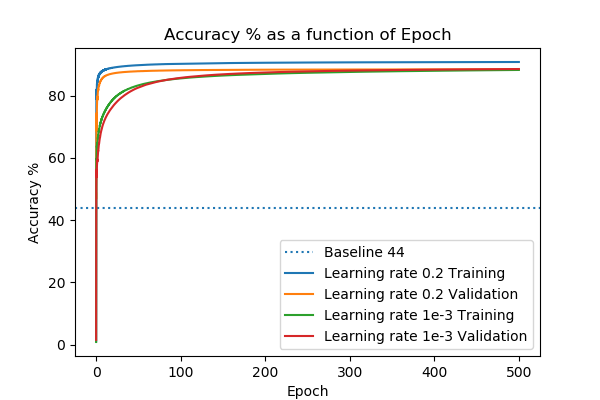
\includegraphics{parts/appendix/reports-papud/2018_07_24-Learning_rate_optimisation_effect/accuracy.png}
\caption{accuracy}
\end{figure}

\subsection{Conclusion}

The new learning rate is better than the previous one, it will be kept.

\subsection{Improvements and next
steps}

{[}OPTIONAL{]} Use inline optimisation to update the learning rate every
set number of epochs (once convergence is reached).
